% Quiz 6: selected questions and source notes are in q6-draft-261-II2026.md.
\documentclass[12pt]{exam}
\usepackage{amsthm}
\usepackage{bm}
\usepackage{libertine}
\usepackage[utf8]{inputenc}
\usepackage[margin=0.5in]{geometry}
\usepackage{amsmath,amssymb}
\usepackage{multicol}
\usepackage[shortlabels]{enumitem}
\usepackage{siunitx}
\usepackage{physics}
\usepackage{booktabs}
\usepackage{graphicx}
\usepackage{pgfplots}
\usepackage{listings}
\usepackage{tikz}
\usepackage{tikz-3dplot}

\bmdefine{\ii}{i}
\bmdefine{\jj}{j}
\bmdefine{\kk}{k}
\newcommand{\te}{\theta}
\newcommand{\cC}{\mathcal{C}}
\newcommand{\word}[1]{\quad\text{#1}\quad}

\pgfplotsset{width=10cm,compat=1.9}
\usepgfplotslibrary{external}
\tikzexternalize

\newcommand{\class}{Math 261-001}
\newcommand{\examnum}{Quiz 6}
% Date assumed from the weekly Friday schedule; adjust if needed.
\newcommand{\examdate}{October 9}

\begin{document}
\pagestyle{plain}
\thispagestyle{empty}

\noindent
\textbf{\class}\\
\textbf{\examnum}, \textbf{\examdate}

\setlength{\tabcolsep}{3.5cm}
\renewcommand{\arraystretch}{1.5}
\setlength\extrarowheight{1cm}
\begin{tabular}{ |c|c| }
 \hline
 Name   & CSU ID \#  \\
 \hline
\end{tabular}

\vspace{10pt}

Choose and answer \textbf{exactly two} of the four problems. If you attempt
more than two, only the first two will be graded. Write your final answers
in the boxes provided. Only answers in the boxes will be graded.
You may use the surrounding space for scratch work. Each problem is worth
the same number of points.

\begin{enumerate}

% Adapted from UCR Lista 5, exercise 1.9: shortlist A.
\item Use spherical coordinates to evaluate
\[
  I=\iiint_E\frac{dV}{(x^2+y^2+z^2)^{3/2}},
\]
where $E$ is the part of the shell $1\leq x^2+y^2+z^2\leq4$
satisfying $z\geq\sqrt{x^2+y^2}$.
Here $\varphi$ is measured from the positive $z$-axis, and $\theta$
is the azimuthal angle in the $xy$-plane.

\vfill
\begin{flushright}
\framebox(250,50){}
\end{flushright}

% Adapted from UCR Lista 6, exercise 1.4, with a fly and scent interpretation.
\item A fly follows the path $C$ given by
\[
  \vec r(t)=(\cos t,\sin t,2+\cos t+\sin t),
  \qquad0\leq t\leq2\pi.
\]
The scent intensity is $\sigma(x,y,z)=\sqrt{1+(x-y)^2}$.
Compute its scent-weighted flight length $S=\displaystyle\int_C\sigma\,ds$.

\vfill
\begin{flushright}
\framebox(250,50){}
\end{flushright}

\newpage

% Adapted from Moodle 009, ILPD-V1, question 11721830.
\item Compute $\displaystyle\int_C\vec F\cdot d\vec r$, where
\[
  \vec F(x,y)=\left(\frac{y\cos x}{x^2},-\frac{\sin x}{2x}\right),
  \qquad
  \vec r(t)=(t,t^2),\quad \frac\pi2\leq t\leq\pi,
\]
and $C$ is traversed in the direction of increasing $t$.

\vspace{0.8cm}
\vfill
\begin{flushright}
\framebox(250,50){}
\end{flushright}

% Original graphical question. No separate tangent vectors or color cues.
\item For the oriented piece of $C$ inside each dashed square A, B, and C,
is the contribution to $\int_C\vec F\cdot d\vec r$
\textbf{positive}, \textbf{negative}, or \textbf{zero}?
Use the direction arrows on $C$ and the dashed field arrows.
The indicated alignment holds along each highlighted piece.

% Keep the diagram at its tested print size and put the sign boxes beside it.
% With no stretch below Question 4, the freed page height goes to Question 3.
\medskip
\noindent\begin{minipage}[c]{0.65\linewidth}
\centering
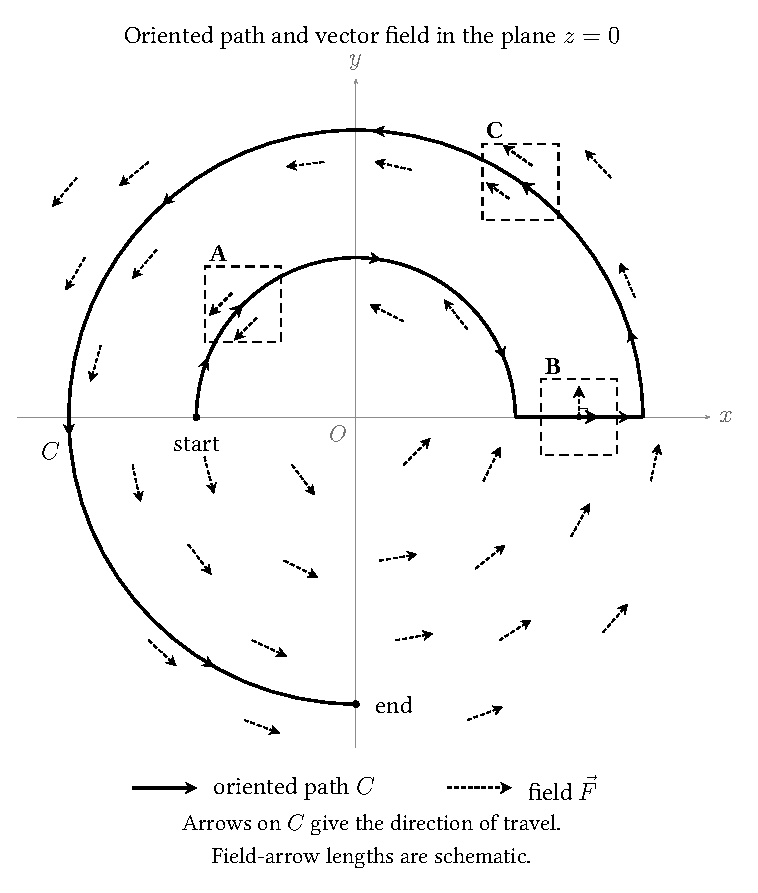
\includegraphics[width=10.7cm]{figures/q6-field-signs.pdf}
\end{minipage}\hfill
\begin{minipage}[c]{0.30\linewidth}
\centering
A: \raisebox{-0.4\height}{\framebox(100,35){}}\par
\vspace{0.8cm}
B: \raisebox{-0.4\height}{\framebox(100,35){}}\par
\vspace{0.8cm}
C: \raisebox{-0.4\height}{\framebox(100,35){}}
\end{minipage}

\end{enumerate}

\end{document}
